\documentclass[format=sigconf]{acmart}
\usepackage{algorithm}
\usepackage{algpseudocode}
\usepackage{caption}
\usepackage{enumitem}
\usepackage{graphicx}

\def\bif{\bf if~}
\def\belif{{\bf else if~}}
\def\bthen{{\bf then predict~}}
\def\belse{{\bf else predict~}}
\def\band{{\bf ~and~}}
\def\ie{{\it i.e.},~}
\def\eg{{\it e.g.},~}

\setcopyright{acmlicensed}

% DOI
%\acmDOI{10.1145/3097983.3098047}

% ISBN
%acmISBN{978-1-4503-4887-4/17/08}

%Conference
\acmConference{SysML '18}{February 15-16, 2018}{Stanford, CA}
\acmYear{2018}
\copyrightyear{2018}

\fancyhead{}
\settopmatter{printacmref=false} % Removes citation information below abstract
\renewcommand\footnotetextcopyrightpermission[1]{} % removes footnote with conference information in first column
%\pagestyle{plain} % removes running headers

\begin{document}

\title{Systems Optimizations for Learning Certifiably Optimal Rule Lists}
\author{Nicholas Larus-Stone}
\affiliation{%
 \institution{Computer Lab, University of Cambridge}
% \city{Cambridge}
% \state{UK}
}
\email{nl363@cl.cam.ac.uk}

\author{Elaine Angelino}
\affiliation{%
  \institution{EECS, UC Berkeley}
%  \city{Berkeley} 
%  \state{CA} 
%  \postcode{94720}
}
\email{elaine@eecs.berkeley.edu}

\author{Daniel Alabi, Margo Seltzer}
\affiliation{%
 \institution{SEAS, Harvard University}
% \city{Cambridge}
% \state{MA}
% \postcode{02138}
\streetaddress{\{alabid@g, margo@eecs\}.harvard.edu}
}

\author{Cynthia Rudin}
\affiliation{%
  \institution{Duke University}
%  \city{Durham}
%  \state{NC} 
%  \postcode{27708}
}
\email{cynthia@cs.duke.edu}

\setlength{\abovedisplayskip}{3pt}
\setlength{\belowdisplayskip}{-10pt}
\setlength{\textfloatsep}{8pt}

\maketitle

\section{Introduction}
Decision trees are an extremely influential prediction technique in AI.
They are interpretable, simple to store, and easy to use \cite{BreimanFrOlSt84}.
However, not enough work has been done on speeding up the creation of decision trees for large datasets.
As big data becomes even more common in machine learning applications, decision trees risk falling in disuse due to computationally prohibitive construction costs.
This work focuses on a set of optimizations that aids with the construction of a specific subset of decision trees: one-sided decision trees, also known as decision lists or rule lists \cite{Rivest87}.
Our goal is to find the rule list that is provably optimal with respect to our objective function, the regularized empirical risk, for a given set of pre-mined rules.
Our algorithm, Certifiably Optimal RulE ListS (CORELS), uses a combination of tight bounds and systems optimizations to achieve reasonable runtimes for moderately sized real datasets (Implementation at \textbf{\url{https://github.com/nlarusstone/corels}}) \citep{AngelinoLaAlSeRu17-kdd, AngelinoLaAlSeRu17}.

Finding the optimal rule list from a set of rules is an computationally hard combinatorial problem with no polynomial-time approximation.
Most decision tree construction strategies solve this by quickly finding an approximate through greedy  methods \citep{BreimanFrOlSt84, Quinlan93}.
Other fields solve similar computationally hard combinatorial problems through the use of branch-and-bound \citep{Clausen99}.
Traditionally, branch-and-bound has only been applied to small problems because the search space is otherwise enormous, even when tight bounds allow for the pruning of the space.
Our use of a branch-and-bound search strategy and the full description of CORELS, including proofs of our bounds, can be found in our previous work \cite{AngelinoLaAlSeRu17, ErtekinRu17}.
Unlike prior greedy approaches, branch-and-bound allows us to find the optimal rule list and certify its optimality.

\begin{figure}[ht!]
\vspace{-2mm}
\begin{algorithmic}
\State \bif $(age = 18-20) \band (sex = male)$ \bthen $yes$
\State \belif $(age = 21-22) \band (priors = 2-3)$ \bthen $yes$
\State \belif $(priors > 3)$ \bthen $yes$
\State \belse $no$
\end{algorithmic}
\caption{Example optimal rule list that predicts two-year recidivism for the ProPublica COMPAS dataset (122 rules), found by CORELS, across 10 cross-validation folds.
%
The rule list shown is representative of~7 folds.
Each of the remaining solutions is the same or similar to one of these, with prefixes containing the same rules, up to a permutation, and the same default rule.
}
\label{fig:recidivism}
\end{figure}

A rule list is composed of an ordered list of rules, an example of which can be seen in Fig \ref{fig:recidivism}.
Rules are features or conjunctions of features that uniformly classify a subset of the observations.
We generate rule lists by adding a rule to the end of a pre-existing rule list.
For a given rule list, any longer rule list that starts with the same rules will make the same mistakes as the shorter one.
To encapsulate this relationship, we call the original rule list a parent and the longer rule list a child.
We calculate both how many observations the list incorrectly classifies as well as a lower bound on the number of mistakes made by any child rule lists.
Calculating each of these metrics from scratch each time would be inefficient; instead, metrics are calculated incrementally using metadata recorded for parent rule list.
The incremental computation takes advantage of a specialized, space-efficient prefix tree by building off of previous computation of parent rule lists.
We systematically search the entire space of rule lists, evaluating them in an order specified by our priority metric; for example, a breadth-first search priority metric entails us examining shorter rule lists before longer ones.

Our objective function combines the number of incorrectly classified observations, normalized to measure misclassification error, with a regularization term that penalizes longer rule lists.
The maximum number of mistakes provides a bound for how well the children of a rule list could ever perform.
Using those two metrics, we are able to compare the future performance of all of a rule list's children to the current best rule list we have seen so far.
If the best future performance is worse than the performance of a rule list we have already seen, then we know it can not be the optimal rule list, thus we can prune it.
We also proved a suite of additional algorithmic bounds that interact to aggressively prune the search space.
In our implementation, we exploit these bounds via several data structures.  
Together with additional systems optimizations, our approach efficiently searches the space of rule lists to find a provably optimal solution.

In our earlier work, we performed a number of experiments on the ProPublica COMPAS dataset \cite{LarsonMaKiAn16} and predicted whether or not an individual would recidivate within 2 years.
This dataset contains 122 rules ; therefore, a brute force search of all possible rule lists up to length 10 would require evaluating ${5.0 \times 10^{20}}$ rule lists.
Due to our algorithmic bounds, CORELS only examines 28 million rule lists, a reduction of ${1.8 \times 10^{13}}$.
Between the numerous bit vector operations and the pruning required, a non-optimized implementation of our algorithm would not complete.
However, in our final implementation, each evaluation takes only 1.3~$\mu$s, allowing us to complete that moderately sized problem in 36s.
Systems optimizations, even on just a single processor, allow us to solve a computationally hard problem of reasonable size in under a minute.

\section{Implementation}
Our algorithm is feasible due to the use of three core data structures.
Firstly, we use a prefix tree to represent the search space.
The incremental nature of our algorithm requires that we store rule lists that we examined but did not discard.
The prefix tree structure allows us to easily access values in a parent rule list to calculate bounds for a new rule list.
Next, we implement our scheduling policy with a priority queue.
Finally, in order to implement one of our critical bounds, we use a symmetry-aware map.
It allows us to easily compare and prune rule lists that are created from the same set of rules (\ie permutations of each other).

%\begin{itemize}[leftmargin=*, itemsep=0.8\baselineskip]
%\item 
To support incremental execution, we use a prefix tree to cache rule lists that we have already evaluated and have not pruned.
Each node in the tree represents a rule, so any rule list can be reconstructed by following a path from the root to a leaf in the tree.
The node stores metadata to aid in the computation of our bounds including: the lower bound, objective value, and a list of unpruned children.
Nodes also have parent pointers, so each node is created incrementally by using the parent's bounds to calculate the new bounds.
This structure also means that a rule list can be represented and passed around as a pointer to a single node in the tree or as an ordered list of rules.
In most cases the pointer is more efficient, though the list representation is useful as a hashable index.

%\item 
We represent our worklist with a priority queue.
This allows us to easily try different exploration orders simply by changing the priority metric.
We implement breadth-first search (BFS), depth-first search (DFS), and a priority search that can take a custom metric.
Our implementation supports ordering by the lower bound and the objective, though any function that maps a prefix to a real value in a stable manner would work.
In general, we find that ordering by lower bound (best-first search) yields the best results on most datasets.

%\item 
In order to take advantage of the symmetry inherent to our problem, we had to design a novel structure called a symmetry-aware map.
We use this map to keep track of the best possible permutation of a given set of rules.
When a new permutation of that set of rules is encountered, we only add the new permutation to our prefix tree if it is strictly better than the permutation we already have stored.
We experimented with multiple key types that could represent permutations of rule lists and found that a simple optimization of the key type led to a 3x reduction in memory usage for the map \cite{Larus-Stone17}.

%\item 
An important part of our implementation is that we calculate accuracy and other metrics by using bit vector operations.
Each rule is represented as a bit vector where each individual is 1 if the rule applies to that individual and 0 otherwise.
We use the high performance bit vector rule library from an earlier work \cite{YangRuSe16}.
The implementation uses the GMP multiple-precision library to hold the bit vectors and perform operations on them.
This is more efficient than built-in C++ constructs such as a vector of bools or a bitset.
Profiling of CORELS has shown that the majority of algorithm's execution time is spent performing the bit vector operations necessary to calculate our bounds.
Thus, speeding up these computations would accelerate the execution of our algorithm and is a promising direction for future work.
%\end{itemize}
%\vspace{0.5\baselineskip}

Each one of these structures and optimizations is critical for the success of our algorithm.
For example, we briefly experimented with a stochastic search policy that did not use a queue at all but instead followed random paths from the queue to a leaf.
However, this search strategy performed worse than any strategy involving our queue, so we proceeded only by using the queue.
Fig \ref{fig:ablation} shows another example of how important data structure design is for solving hard problems such as ours.
It demonstrates how simply adding the symmetry-aware map can turn a computationally intractable problem into an execution that completes in under 60s.

\begin{figure}[t!]
\begin{center}
% left lower right upper
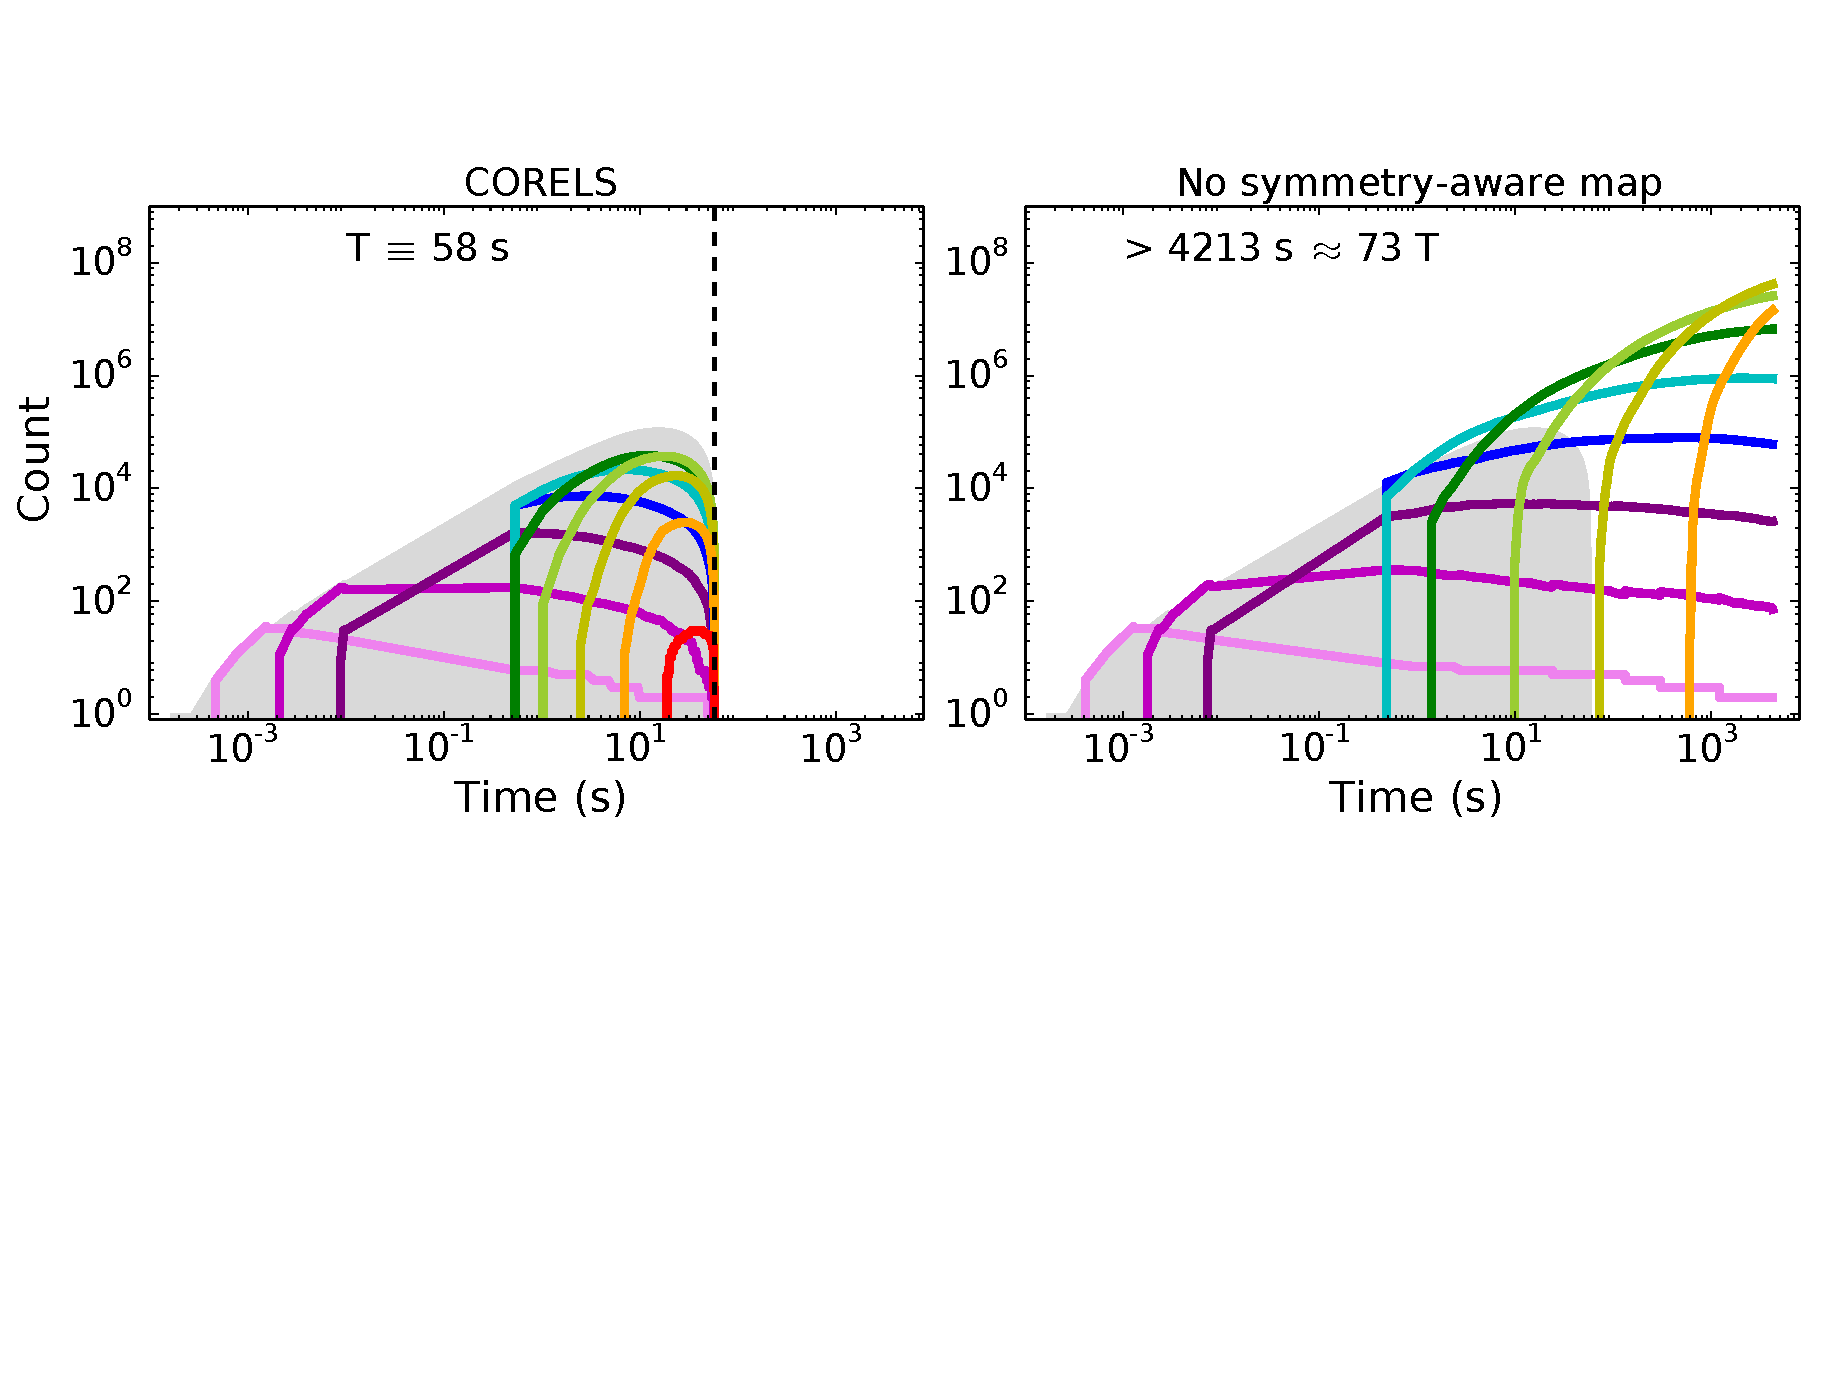
\includegraphics[trim={4mm 0mm 0mm 0mm}, width=0.48\textwidth]{figs/sysml_ablation-queue.pdf}
\end{center}
\vspace{-5mm}
\caption{Summary of the queue's contents, for full CORELS and CORELS without the symmetry-aware map on the NYCLU dataset (29,595 samples, 46 rules)  \citep{nyclu:2014}.
Each color line represents a different length of rule list, while the gray area is the shape of our baseline execution.
The execution without the symmetry-aware map was terminated due to memory consumption without certifying the optimality of the best rule list it found.
}
\label{fig:ablation}
\end{figure}

\section{Conclusion}
We demonstrated that it is possible to learn certifiably optimal rule lists, but only through a combination of algorithmic bounds, systems optimizations, and efficient data structures.
While much of the theory in this area was developed in the 1980s and 1990s, to the best of our knowledge there have been few dedicated systems approaches that take advantage of modern hardware to work on real problems.
Future work on CORELS involves parallelizing the algorithm both for a single machine with many cores and for distributed systems.
Additionally, further scaling could be realized by porting the algorithm to an FPGA.
We are optimistic that other classic AI algorithms may benefit from investigations of systems level optimizations.

\bibliographystyle{plainnat}
%\bibliographystyle{ACM-Reference-Format}
\bibliography{sys_refs}

\end{document}
